\section{Speicher}
\label{sec:speicher}

\textbf{Begriffe}:
\begin{items}
	\item \underline{Hauptspeicher}: "`Gedächtnis"' des Rechners. Beinhaltet Programme und Daten, die jederzeit und sofort (\emph{random access}) zur Verfügung stehen müssen
	\begin{figure}[H]\centering\label{Hauptspeicher-Struktur}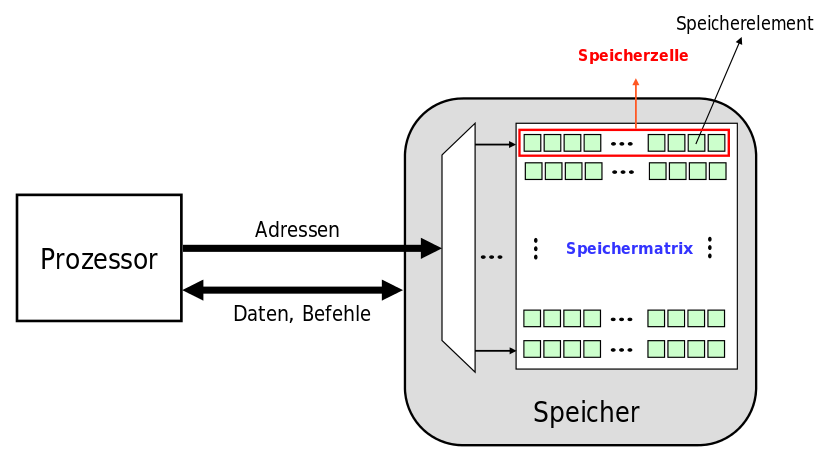
\includegraphics[width=0.33\textwidth]{Hauptspeicher-Struktur}\end{figure}

	\item \underline{Speicherelement}: 1 Bit Speicher

	\item \underline{Speicherzelle}: feste Anzahl von Speicherelementen, auswählbar durch eindeutige Adresse. 8,16,32,\dots Bit

	\item \underline{Speicherwort}: maximale Anzahl an Speicherelementen, die in einem Buszyklus zwischen Mikroprozessor und Speicher übertragen werden können \( \leadsto \) Speicherwortbreite \( = \) \emph{Datenbusbreite}

	\item \underline{Wahlfreier Zugriff}: Jede Speicherzelle kann direkt angesprochen werden (ohne andere Zellen ansprechen zu müssen), Selektion über Adressdecoder

	\item \underline{Speicherorganisation}: Definition über Anzahl \( n \) der Zeilen und Anzahl \( m \) der Speicherelemente pro Zeile, z.B. 16-MBit-DRAM mit Organisation 4Mx4/2Mx8/1Mx16

	\item \underline{Kapazität}: Informationsmenge, die im Speicher untergebracht werden kann (\( n*m \) Bit)

	\item \underline{Arbeitsgeschwindigkeit}:
	\begin{enumeration}
		\item \textbf{Zugriffszeit} (\emph{}access time): maximale Zeit zwischen Anlegen einer Speicheradresse imd Ausgabe der gewünschten Daten

		\item \textbf{Zykluszeit} (\emph{cycle time}): minimale nötige Zeit zwischen zwei hintereinanderfolgenden Adressenaufschaltengen an den Speicher

		\begin{figure}[H]\centering\label{ZykluszeitZugriffszeit}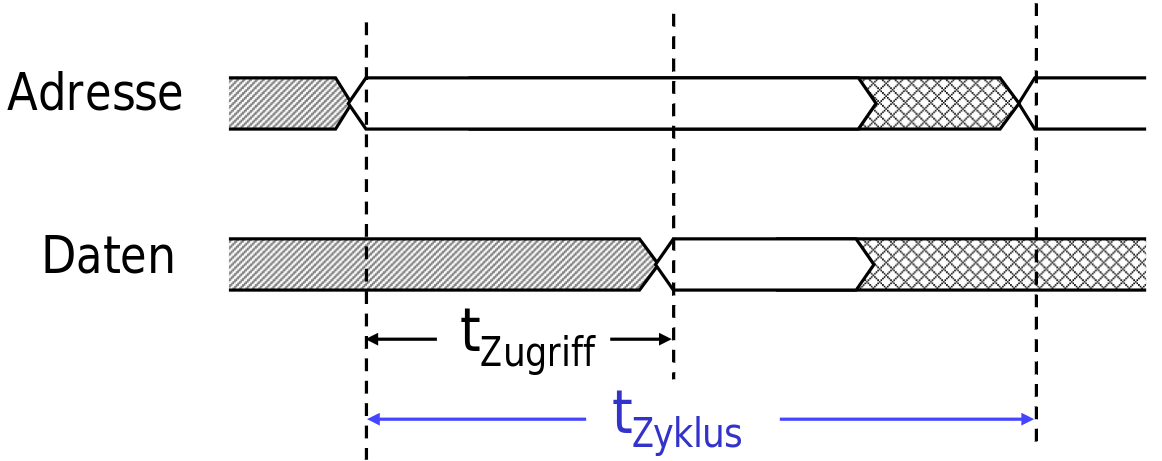
\includegraphics[width=0.33\textwidth]{ZykluszeitZugriffszeit}\end{figure}
	\end{enumeration}
\end{items}

\textbf{Speicherklassifizierung}:
\begin{figure}[H]\centering\label{Speicherklassifizierung}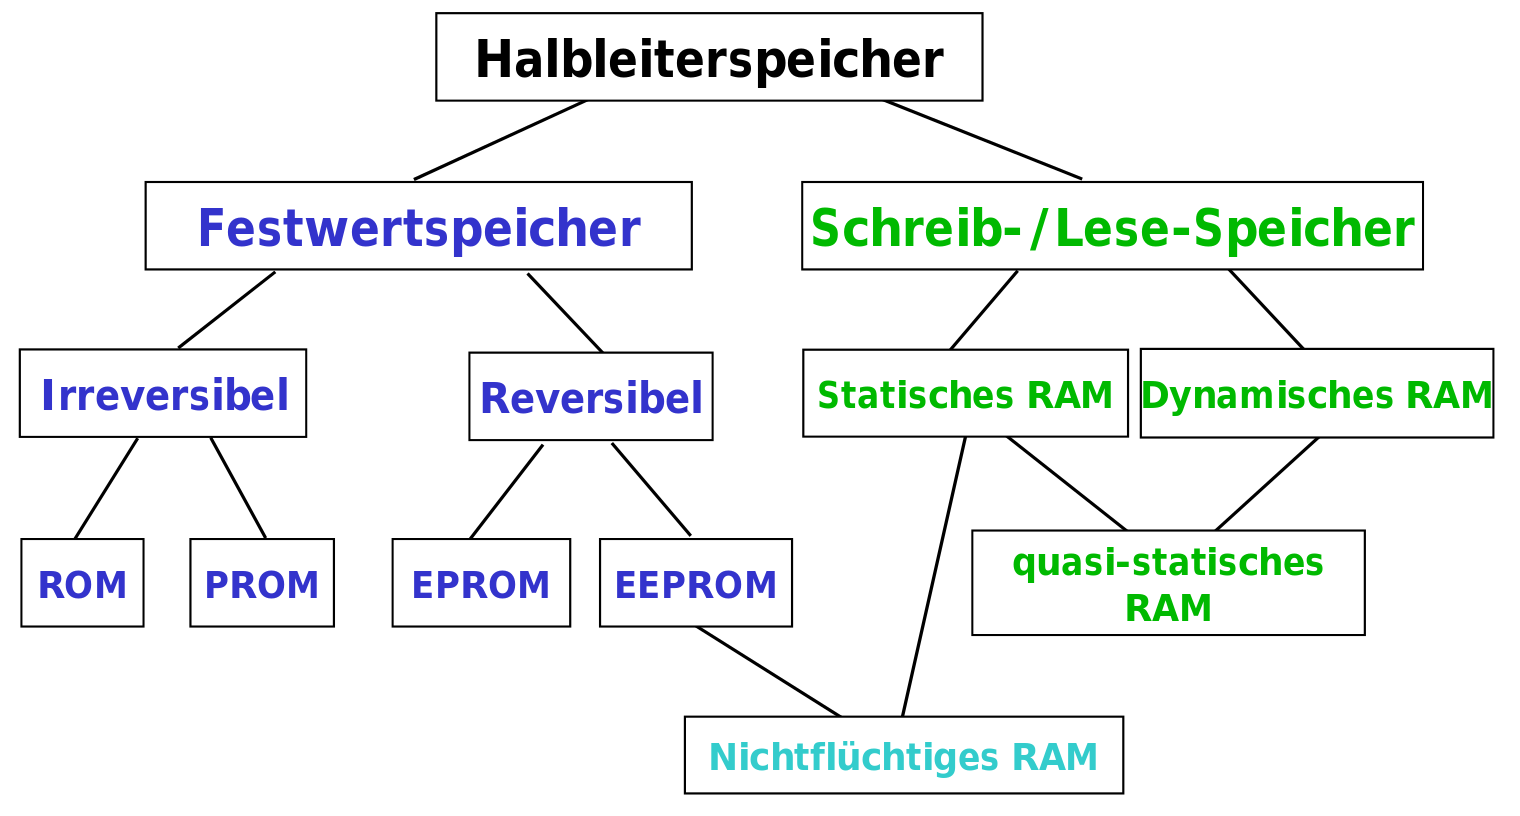
\includegraphics[width=0.33\textwidth]{Speicherklassifizierung}\end{figure}

\newpage

\textbf{Transistor (MOSFET)}:
\begin{items}
	\item Eine Spannung an einem \emph{Gate} regelt, ob Strom zwischen \emph{Source} und \emph{Drain} fließt.
	\item \underline{n-MOS-MOSFET}: Kanal sperrt, wenn keine Spannung anliegt (\emph{selbstsperrend})
\end{items}
\begin{figure}[H]\centering\label{MOSFET}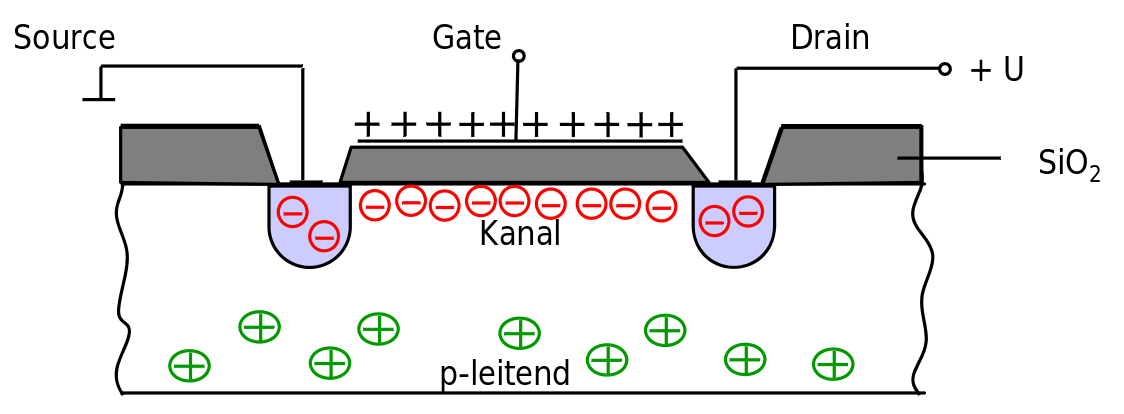
\includegraphics[width=0.33\textwidth]{MOSFET}\end{figure}

\textbf{Speicherzelle -- statisch (SRAM)}:
\begin{items}
	\item Aufgebaut aus zwei kreuzweise rückgekoppelten Invertern und zwei Transistoren zur Ankopplung an Bitleitungen \( \leadsto \) 6-Transistor-Zelle
	\item \underline{Vorteile}: Strom fließt nur zum Umschaltzeitpunkt \( \leadsto \) kein Refresh nötig
	\item \underline{Nachteile}: Hoher Platzverbrauch
\end{items}

\textbf{Speicherzelle -- dynamisch (DRAM)}:
\begin{items}
	\item Aufgebaut aus einer Transistorzelle und einem Kondensator (vergößerte Drain-Zone, von Drain-Kontakt durch dünne Isolierschicht getrennt) \( \leadsto \) Platzverbrauch viermal kleiner als bei SRAM
	\item \underline{Vorteile}: Geriner Platzverbrauch
	\item \underline{Nachteile}: Information geht beim Lesen verloren und muss neu gespeichert werden (\emph{destructive read}), Ladung geht nach einiger Zeit durch Leckströme verloren \( \leadsto \) periodische Auffrischung (\emph{refresh}) nötig
	\item \underline{Lesen}:
	\begin{enumeration}
		\item Leistungskapazität wird vorgeladen (\emph{precharge})
		\item Positive Spannung wird an Gate des Speichertransistors angelegt
		\item Leseverstärker misst Strom am Ende der Bitleitung
	\end{enumeration}
	\item \underline{Schreiben}: 
	\begin{enumeration}
		\item Speichertransistor wird durch Spannung \( U_{GS} \) leitend
		\item Bitleitung auf Masse  \( \leadsto \) Elektronen werden auf Drain-Zone aufgebracht, Kondensator lädt
		\item Bitleitung auf \( U_B \leadsto \) Elektronen von Drain-Zone abgesaugt, Kondensator entlädt 
	\end{enumeration}
\end{items}
\begin{figure}[H]\centering\label{AufbauDRAM}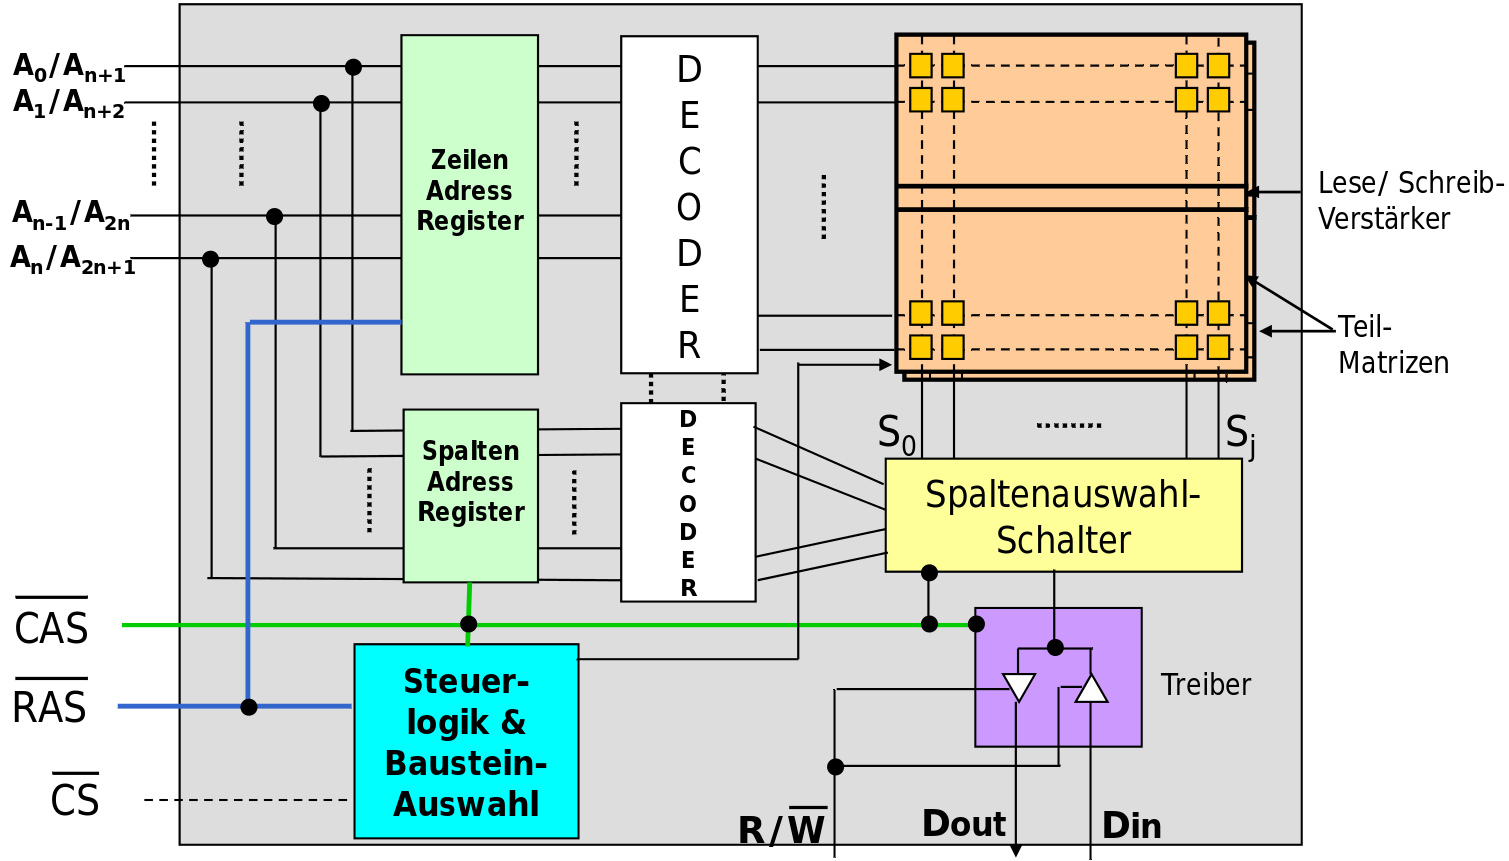
\includegraphics[width=0.5\textwidth]{AufbauDRAM}\end{figure}